\documentclass[11pt]{article}
\usepackage[T1]{fontenc}
\usepackage{lmodern}
\usepackage[margin=1in]{geometry}
\usepackage{amsmath,amssymb,amsthm}
\usepackage{microtype}
\usepackage{tikz}
\usepackage[hidelinks,hypertexnames=false]{hyperref}
\hypersetup{pdftitle={A two-replica proof of the Krenn--Gu conjecture},pdfauthor={}}
\newtheorem{theorem}{Theorem}[section]
\newtheorem{lemma}[theorem]{Lemma}
\newtheorem{corollary}[theorem]{Corollary}
\theoremstyle{definition}
\newtheorem{definition}[theorem]{Definition}
\theoremstyle{plain}
\numberwithin{equation}{section}
\setlength{\parskip}{0.25em}
\title{A two-replica proof of the Krenn--Gu conjecture}
\author{}
\date{September 26, 2026}
\begin{document}
\maketitle
\begin{abstract}
In the graph model of photonic state preparation, the amplitude of a vertex
colouring is a sum of products of complex edge weights over perfect matchings.
The Krenn--Gu conjecture asks whether these weights can cancel every mixed
colouring while retaining at least three monochromatic colourings on more
than four vertices. We prove that they cannot. The main difficulty is that
the existence of a mixed matching alone does not prevent its amplitude from
cancelling. Our argument forces a stronger structure: after parallel edges
with the same endpoint colours are aggregated, every edge is monochromatic
and every active colour forms a perfect matching. A vertex colouring then
has at most one contributing matching, so a known combinatorial obstruction
finishes the proof. The structural argument uses two identical formal copies
of the matching polynomial. Their symmetries impose polynomial identities
that force each supported edge to contribute the entire amplitude of its
colour. Complex weights, parallel edges, and distinct colours at the two
ends of an edge are all allowed. A Lean formalization verifies the normalized
equation-system statement at every even order at least six and every palette
size at least three.
\end{abstract}

\section{Introduction}\label{sec:introduction}

Perfect matchings provide a bridge between graph theory and the preparation
of entangled states with photon-pair sources~\cite{kgz}. Vertices represent output paths,
edges represent pair contributions, and endpoint colours specify the modes.
Selecting one photon at each output corresponds to selecting a perfect
matching. Contributions that induce the same output modes add as complex
amplitudes; they can therefore interfere destructively~\cite{graphs2}. The resulting
existence question was formulated by Krenn, Gu and
Solt\'esz~\cite[Question~1]{kgs}; see also the matching examples
in~\cite[Section~2]{logic}.

For a Greenberger--Horne--Zeilinger (GHZ) target, the desired colourings assign the same colour to every
vertex. All other colourings must have amplitude zero. Graph theory can
force an unwanted matching to exist, but complex weights might cancel its
contribution against other matchings. The proof must therefore explain why
such cancellation cannot satisfy all the target equations simultaneously.
We do this by deriving a structural restriction on the weighted graph itself.

\subsection{Matching amplitudes and the conjecture}\label{sec:graphmodel}

Let \(G=(V,E)\) be a finite loopless multigraph. Each edge \(e=uv\) has
weight \(w(e)\in\mathbb C\) and two endpoint colours \(\chi_u(e),\chi_v(e)\).
We write \([d]=\{1,\ldots,d\}\) for the target palette and
\(\mathcal M(G)\) for the set of perfect matchings of \(G\).
For \(M\in\mathcal M(G)\), let \(e_M(v)\) be its unique edge at \(v\).
The matching induces the vertex colouring
\(v\mapsto\chi_v(e_M(v))\). For a vertex colouring \(\kappa:V\to[d]\), define
\[
 W(\kappa)=
 \sum_{\substack{M\in\mathcal M(G)\\
       \chi_v(e_M(v))=\kappa(v)\ \text{for every }v}}
       \prod_{e\in M}w(e).
\]
An empty sum is zero. We write \(i^V\) for the colouring that is constantly
\(i\). A colouring that is not constant is called mixed. For a matrix \(B\)
and a vertex set \(S\), \(B[S]\) denotes its principal submatrix on \(S\).

In the physical interpretation, these coefficients give the unnormalized
postselected state
\[
 |\psi_G\rangle=\sum_{\kappa:V\to[d]}W(\kappa)
                 \bigotimes_{v\in V}|\kappa(v)\rangle_v.
\]
Here \(|h\rangle_v\) denotes basis mode \(h\) in output path \(v\).
Postselection means conditioning on one photon in each path. The weights
and their matching products are amplitudes, not probabilities. The theorem
concerns the states represented by this matching model.

\begin{definition}[Generalized GHZ condition]\label{def:ghz}
The weighted half-edge-coloured graph satisfies the generalized GHZ condition
on \([d]\) if \(W(i^V)=\tau_i\ne0\) for every \(i\in[d]\), and
\(W(\kappa)=0\) for every mixed vertex colouring \(\kappa:V\to[d]\).
\end{definition}

The usual normalized condition requires \(\tau_i=1\). Our definitions follow
Chandran, Gajjala and Illickan~\cite[Sections~1.1 and~1.4]{cgi}; the
generalized condition permits unequal nonzero amplitudes. We call a colour
\emph{active} when its monochromatic amplitude is nonzero. All colours in
the target palette of Definition~\ref{def:ghz} are therefore active.

\begin{theorem}[Krenn--Gu conjecture]\label{thm:graphmain}
If \(|V|>4\) is even, there is no complex weighted half-edge-coloured
multigraph satisfying the generalized GHZ condition on a palette of size
\(d\ge3\).
\end{theorem}

The theorem concerns this matching model with arbitrary complex weights.
There is no restriction on edge density or on the number of parallel edges.
It suffices to retain three active colours: removing edges with other
endpoint colours leaves every amplitude on the retained palette unchanged.

\subsection{Cancellation and the four-vertex boundary}

Consider the left-hand graph in Figure~\ref{fig:examples}. Both of its
perfect matchings induce the mixed colouring \((a,a,b,b)\). Their weights
are \(1\cdot1\) and \(1\cdot(-1)\), so
\[
 W(a,a,b,b)=1\cdot1+1\cdot(-1)=0.
\]
Thus a zero amplitude does not imply the absence of a matching. This small
graph illustrates cancellation only; it does not satisfy the GHZ condition.
The proof has to use the nonzero monochromatic amplitudes together with
the vanishing of \emph{every} mixed amplitude.

\begin{figure}[htbp]
\centering
\begin{minipage}[t]{0.48\textwidth}
\centering
\begin{tikzpicture}[x=1pt,y=1pt,line width=0.8pt]
\path[use as bounding box] (0,0) rectangle (200,116);
\draw[red!70!black] (45,85)--(145,85);
\draw[blue!75!black] (45,25)--(145,25);
\draw[red!70!black] (45,85)--(45,55) (145,85)--(145,55);
\draw[blue!75!black] (45,55)--(45,25) (145,55)--(145,25);
\foreach \x in {45,145} \foreach \y in {25,85}
  \fill (\x,\y) circle (2pt);
\node at (45,101) {\(1:a\)}; \node at (145,101) {\(2:a\)};
\node at (45,9) {\(3:b\)}; \node at (145,9) {\(4:b\)};
\node at (95,95) {\(1\)}; \node at (95,15) {\(1\)};
\node at (31,55) {\(1\)}; \node at (163,55) {\(-1\)};
\end{tikzpicture}

\small (a) Two contributions to \((a,a,b,b)\):\\
\(\{12,34\}:1\cdot1=1\),
\(\{13,24\}:1\cdot(-1)=-1\).
\end{minipage}\hfill
\begin{minipage}[t]{0.48\textwidth}
\centering
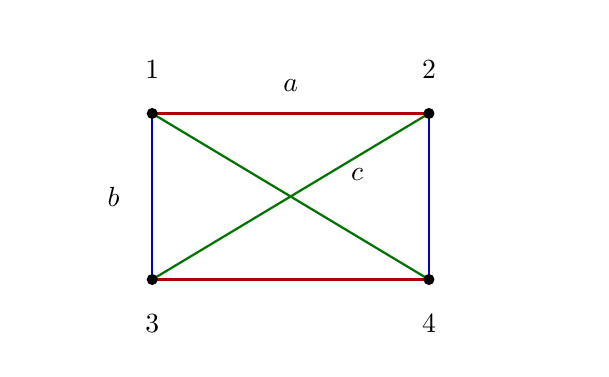
\begin{tikzpicture}[x=1pt,y=1pt,line width=0.8pt]
\path[use as bounding box] (0,0) rectangle (200,116);
\draw[red!70!black] (45,85)--(145,85) (45,25)--(145,25);
\draw[blue!75!black] (45,25)--(45,85) (145,25)--(145,85);
\draw[green!45!black] (45,25)--(145,85) (45,85)--(145,25);
\foreach \x in {45,145} \foreach \y in {25,85}
  \fill (\x,\y) circle (2pt);
\node at (45,101) {\(1\)}; \node at (145,101) {\(2\)};
\node at (45,9) {\(3\)}; \node at (145,9) {\(4\)};
\node at (95,95) {\(a\)}; \node at (31,55) {\(b\)};
\node at (119,63) {\(c\)};
\end{tikzpicture}

\small (b) The four-vertex GHZ construction:\\
\(a:\{12,34\},\ b:\{13,24\},\ c:\{14,23\}\).
\end{minipage}
\caption{The obstruction and the exceptional case. In (a), labels beside
edges are weights and labels at vertices give the inherited colours; the
two vertical edges have different colours at their ends. In (b), all weights
are one. Horizontal, vertical, and diagonal edges have colours \(a,b,c\),
respectively. The diagonal crossing is not a vertex.}
\label{fig:examples}
\end{figure}

The restriction to more than four vertices is necessary. In
Figure~\ref{fig:examples}(b), the three perfect matchings of \(K_4\) are
\[
 \{12,34\},\qquad \{13,24\},\qquad \{14,23\}.
\]
Colour these matchings \(a,b,c\), respectively, and give every edge weight
one. The only induced colourings are \(a^V,b^V,c^V\), each with amplitude
one. Our structural argument will recover precisely the feature visible in
this example: each colour forms a perfect matching. The final graph
obstruction then distinguishes four vertices from larger orders.

\subsection{Related work and contribution}

The graph correspondence originates with Krenn, Gu and Zeilinger~\cite{kgz};
its weighted interference formulation is developed further in~\cite{graphs2}.
The weighted, endpoint-coloured existence question is stated
in~\cite[Question~1]{kgs}. Complex amplitudes distinguish this question from
the purely combinatorial problem of forbidding mixed perfect matchings.

Bogdanov proved the combinatorial obstruction in 2017~\cite{bogdanov};
\cite[Theorem~7]{cgi} records the form we use. Chandran and Gajjala classify
the simple graphs admitting edge colourings in which every perfect matching
is monochromatic, and derive weighted consequences~\cite{cgclass}.
Their separate sparsification theorem excludes dimension
\(d\ge n/\sqrt2\) on simple graphs with \(n>4\), permitting complex
weights and bichromatic edges~\cite[Theorem~8]{cg}. In contrast,
Cervera-Lierta, Krenn and Aspuru-Guzik's SAT exclusions at \((n,d)=(6,3)\)
and \((8,4)\) assume monochromatic edges. Their general Boolean conditions
are necessary support constraints; satisfiability alone does not construct
the complex amplitudes~\cite[Sections~3.1--3.2]{logic}.

In the general weighted multigraph model, Chandran, Gajjala and Illickan
prove the conjecture when the underlying simple graph has vertex
connectivity at most two or maximum degree at most three. Their reduction
also forces a minimum-vertex counterexample to be four-connected
\cite[Theorems~9--11]{cgi}. Their cubic-case proof already obtains a unique
matching for each contributing colouring and then applies Bogdanov's
obstruction~\cite[Section~2.3, Corollary~17]{cgi}. We use that same final
strategy. The contribution here is the algebraic derivation of
monochromatic aggregate edges and degree one in every active colour
without a sparsity assumption.

Recent formal work addresses further cases. A public Lean certificate
artifact exports the complex six-vertex, three-colour statement~\cite{sixvertex}.
Krenn's problem page reports an all-even-order obstruction for \(d\ge n\)
in 2026~\cite{krennstatus}. The AlphaProof Nexus preprint discusses this
research and explicitly lists \(N=d\in\{4,6,10\}\), while citing a
follow-up tensor-algebraic manuscript as in preparation
\cite[Section~4 and reference~38]{nexus}. We distinguish the author-announced
bound from the displayed instances in that preprint; the unavailable
follow-up manuscript is not an input to our proof or a basis for a
comparison of methods.

The standard algebraic ingredients are the pairing formula, polarization,
and scalar orthogonal invariant theory~\cite{isserlis,kraft}. We define and
explain their use below. The matching equations supply the additional
response identities and matrix divisibility that are needed for the
supported-edge identity.

\subsection{Proof overview: forcing one edge per colour}\label{sec:overview}

We first remove an ambiguity caused by parallel edges. For fixed vertices
\(u,v\) and fixed endpoint colours \(i,j\), replace all corresponding
parallel edges by one edge whose weight is their sum. Delete that edge if
the sum is zero. A perfect matching uses at most one edge between \(u\) and
\(v\), so distributivity shows that this operation preserves every
\(W(\kappa)\). All support and uniqueness statements below refer to this
\emph{aggregate graph}. This reduction is also stated in
\cite[page~41:5]{cgi}.

The argument has two structural steps and a short combinatorial conclusion.
We describe the conclusion first far enough to make the role of each
structural step explicit.

\paragraph{Step 1: every remaining edge has equal endpoint colours.}
Lemma~\ref{lem:diagonal} proves that every aggregate weight with distinct
endpoint colours is zero. After this reduction, fix an active colour and
write \(B_{pq}\) for its weight on the edge \(pq\). A supported edge means
one with \(B_{pq}\ne0\). Let \(\beta\ne0\) be the amplitude of the
monochromatic colouring in this colour.

\paragraph{Step 2: each supported edge contributes the entire amplitude.}
For an edge \(pq\), define its matching subtotal
\[
 C_{pq}=\sum_{\substack{M\text{ a perfect matching of this colour}\\pq\in M}}
              \prod_{e\in M}w(e).
\]
The central identity, proved in Theorem~\ref{thm:endpoint}, is
\[
 \boxed{C_{pq}=\beta\quad\text{whenever }B_{pq}\ne0.}
\]
Its consequence is immediate. Every perfect matching uses exactly one edge
at a fixed vertex \(p\). If \(\deg_B(p)\) counts the supported edges of
this colour at \(p\), then
\[
 \beta=\sum_{q:\,B_{pq}\ne0}C_{pq}=\deg_B(p)\,\beta.
\]
Since \(\beta\ne0\), we obtain \(\deg_B(p)=1\). This applies to every
vertex and every active colour: each colour graph is a perfect matching.
In particular, the conclusion uses complex amplitudes directly and requires
no positivity argument.

\paragraph{Step 3: a mixed matching can no longer cancel.}
Given a vertex colouring \(\kappa\), its colour at each vertex specifies
the only possible incident edge in a contributing matching. Consequently
there is at most one such matching. If it exists, its weight is a product
of nonzero edge weights and hence is nonzero. But three monochromatic
perfect matchings of distinct colours on more than four vertices force a
mixed perfect matching~\cite[Theorem~7]{cgi}. Its nonzero amplitude
contradicts the GHZ condition. We include the graph argument in
Section~\ref{sec:graph}.

\paragraph{Where the algebra enters.}
The difficult work is to establish Steps 1 and 2. A matching subtotal can be
written as
\[
 C_{pq}=B_{pq}\,\mathrm{haf}\bigl(B[V\setminus\{p,q\}]\bigr),
\]
where the hafnian is the sum of products over perfect matchings on the
remaining vertices. Thus Step 2 is an identity relating a full matching
sum to a sum with two vertices removed. The remaining graph is not assumed
to satisfy any GHZ condition; the identity must follow from the equations
on the original graph.

We obtain such identities by taking two identical formal copies of the
matching polynomial. Mixing the copies preserves their pairing data, while
certain alternating expressions change sign. This yields vanishing
identities that are not visible in a single matching sum. A second use of
the symmetry restricts an auxiliary matrix to a small family of polynomial
forms. The original matching equations then impose differential equations
on their coefficients. A polynomial of positive degree cannot satisfy
\(p'+\delta p=k\) when \(\delta\ne0\) and \(k\) is constant: its
highest-degree term would have nothing to cancel. This finite-degree
argument gives the supported-edge identity.

Section~\ref{sec:model} develops the pairing language from a four-factor
example. Sections~\ref{sec:higher} and~\ref{sec:diagonal} establish Step 1;
Section~\ref{sec:endpoint} proves the identity in Step 2. The final two
steps above are completed in Sections~\ref{sec:matching} and~\ref{sec:graph}.
Section~\ref{sec:scope} states the precise formalization scope.

\section{Algebraic formulation and formal pairings}\label{sec:model}

\subsection{Encoding a matching sum}

Our first algebraic operation enforces the matching rule: a vertex may be
used only once. Associate a variable \(x_{v,i}\) with colour \(i\) at
vertex \(v\), and set every product \(x_{v,i}x_{v,j}\) to zero. Thus a
product of edges sharing a vertex vanishes, regardless of their colours.
Products of vertex-disjoint edges survive.

Write \(n=|V|\) and fix an ordering of \(V\).
Let \(A_{uv}(i,j)\) be the sum of the weights of edges whose endpoint colours
are \(i\) at \(u\) and \(j\) at \(v\), as in the aggregation in
Section~\ref{sec:overview}. When we reverse the vertex order, we use
\(A_{vu}(j,i)=A_{uv}(i,j)\). The algebra and its edge polynomial are
\[
 \begin{aligned}
 \mathcal A_V&=\mathbb C[x_{v,i}:v\in V,\ i\in\{a,b,c\}]
       \big/\bigl(x_{v,i}x_{v,j}:v\in V,\ i,j\in\{a,b,c\}\bigr),\\
 A&=\sum_{u<v}\sum_{i,j\in\{a,b,c\}}A_{uv}(i,j)x_{u,i}x_{v,j}.
 \end{aligned}
\]
Every surviving term in its divided top power chooses each vertex exactly once.
The division by \((n/2)!\) removes the ordering of the chosen edges. Thus the
coefficient of \(\prod_v x_{v,\kappa(v)}\) is exactly \(W(\kappa)\).
We use \(A^{[j]}=A^j/j!\) for these divided powers. For one colour on four
vertices, the coefficient is the familiar three-term matching sum
\[
 \mathrm{haf}(B)=B_{12}B_{34}+B_{13}B_{24}+B_{14}B_{23}.
\]
In general, \(\mathrm{haf}(B[S])\) denotes the corresponding sum on the
even vertex set \(S\), with value one when \(S\) is empty.

We may therefore express the ternary instance of
Definition~\ref{def:ghz} as follows. Write \(a_v,b_v,c_v\) for the three
coordinates at \(v\), and \(h^S=\prod_{v\in S}h_v\).

\begin{theorem}[Algebraic form of Theorem~\ref{thm:graphmain}]\label{thm:main}
Let \(V\) have even cardinality \(n>4\). In the algebra \(\mathcal A_V\),
let \(A\) be any quadratic involving only distinct vertices, with arbitrary
complex coefficients. Then
\begin{equation}
 A^{[n/2]}=\tau_a a^V+\tau_b b^V+\tau_c c^V,
 \qquad \tau_a\tau_b\tau_c\ne0
 \tag{1}\label{eq:target}
\end{equation}
is impossible.
\end{theorem}

The coefficient interpretation just proved identifies this statement with
the graph theorem after palette restriction. The algebra keeps the original
complex weights, including all aggregate bichromatic weights.

\subsection{Rows, colour words, and coefficients}\label{sec:rows}

We use the same construction on any subset \(S\subseteq V\):
\(\mathcal A_S\) has variables \(x_{v,h}\) for \(v\in S\) and
\(h\in\{a,b,c\}\), with the same rule that two variables at one vertex
have product zero. Its degree-one elements are called \emph{rows}. Thus
\[
 L=\sum_{v\in S}\sum_{h\in\{a,b,c\}}L_v(h)x_{v,h},
 \qquad L_v(h)\in\mathbb C.
\]
A row is a list of coefficients, one for each vertex and colour, written as
a linear polynomial. The term comes from the edges incident on one fixed
vertex; the precise incident row is defined in Section~\ref{sec:rootrows}.

A \emph{colour word} on \(S\) is simply a colouring
\(\kappa:S\to\{a,b,c\}\). It labels the monomial
\(x^\kappa=\prod_{v\in S}x_{v,\kappa(v)}\). These monomials form a basis
of the degree-\(|S|\) part of \(\mathcal A_S\), which we denote by
\(\mathcal T_S\). An element \(F\in\mathcal T_S\) is a finite array of
colouring coefficients, also called a \emph{tensor} in the proof. We write
\([\kappa]F\), or equivalently \(F(\kappa)\), for the coefficient of
\(x^\kappa\) in \(F\). This is coefficient extraction, not evaluation of
the polynomial at a point. In particular, \([h^S]F\) selects the constant
colouring of colour \(h\).

A \emph{binary projection} retains only two chosen colours at every vertex:
set the variables of the third colour to zero. A \emph{binary word} uses at
most those two colours. These operations will let us test selected
coefficients of the original three-colour equations. We denote the projection
onto colours \(h,k\) by \(\pi_{hk}\).

\subsection{Normalizing nonzero target amplitudes}\label{sec:normalization}

\begin{lemma}[Normalization of pure amplitudes]\label{lem:normalization}
A fixed half-edge-coloured graph admits weights satisfying the generalized
GHZ condition if and only if it admits weights satisfying the normalized
condition with every pure amplitude equal to one. The rescaling between
these assignments preserves which edge weights are nonzero.
\end{lemma}

\begin{proof}
The written argument permits arbitrary nonzero \(\tau_i\); the formal
interface uses unit pure amplitudes. To relate them, fix a vertex \(r\).
Multiply each edge incident on \(r\), with colour \(i\) at that endpoint,
by \(\tau_i^{-1}\). Every perfect matching contains exactly one such edge,
so the new amplitude is
\[
 W'(\kappa)=\tau_{\kappa(r)}^{-1}W(\kappa).
\]
Every pure amplitude becomes one and every mixed amplitude remains zero.
The converse follows directly from the generalized definition.
\end{proof}

This is an alternative realization of the normalization equivalence in
\cite[Lemma~14]{cgi}, obtained by rescaling at just one vertex. It changes
edge weights and preserves existence. It is distinct from dividing a quantum
state by its norm and need not be a unitary operation.

\subsection{Formal pairings: a four-factor example}\label{sec:pairings}

A second algebraic description lets us exploit symmetry. Start with an
index set \(\Lambda\), formal commuting symbols \(Z_\lambda\) for
\(\lambda\in\Lambda\), and a symmetric table of complex numbers
\(C_{\lambda\mu}=C_{\mu\lambda}\). Declare the \emph{pairing}
\(\langle Z_\lambda,Z_\mu\rangle_C=C_{\lambda\mu}\), and extend it
bilinearly to linear combinations of symbols. Bilinear means linear in
both arguments, without complex conjugation.

On the ordinary polynomial ring \(\mathbb C[Z_\lambda:\lambda\in\Lambda]\),
define a linear functional \(\mathcal W_C\), called the \emph{formal Wick
functional}, by summing over pairings of the labelled factor occurrences:
\[
 \mathcal W_C(Z_{\lambda_1}\cdots Z_{\lambda_{2r}})
 =\sum_{M\in\mathcal M(\{1,\ldots,2r\})}
       \prod_{\{i,j\}\in M}C_{\lambda_i\lambda_j}.
\]
Here \(\mathcal M(\{1,\ldots,2r\})\) is the set of partitions of the
\(2r\) positions into unordered pairs, equivalently the perfect matchings
on those positions. For four factors this definition says
\[
 \mathcal W_C(Z_1Z_2Z_3Z_4)
 =C_{12}C_{34}+C_{13}C_{24}+C_{14}C_{23}.
\]
An odd number of factors has value zero, and \(\mathcal W_C(1)=1\).
Repeated symbols still occupy distinct positions in the pairing sum.

The table entries are traditionally called \emph{covariances}, and values
of \(\mathcal W_C\) are called \emph{moments}. Here both terms refer only
to the displayed finite sums. No probability distribution, expectation,
positivity, or invertibility is assumed. We can also use polynomial
parameters as entries and apply the same definition coefficientwise.
We use the pairing polynomial appearing in Isserlis's formula
\cite[Section~2, equations~(5)--(6)]{isserlis} as an algebraic definition.
The extension to arbitrary complex pairing tables is part of this definition;
it does not require a probabilistic realization of the table.

For a quadratic matching polynomial \(R\) on a vertex set \(S\), take
\(\Lambda=S\times\{a,b,c\}\). The entry
\(C_{(v,h),(w,k)}\) is the coefficient of \(x_{v,h}x_{w,k}\) in \(R\)
when \(v\ne w\), and is zero when \(v=w\). For even \(|S|=2r\),
\[
 [\kappa]R^{[r]}
 =\mathcal W_C\!\left(\prod_{v\in S}Z_{v,\kappa(v)}\right).
\]
Both sides enumerate the same matchings. This identity is the bridge
between the two algebraic descriptions.

\paragraph{The two kinds of variables have different rules.}
Lower-case \(x_{v,h}\) belong to \(\mathcal A_S\) and obey the
one-use-per-vertex rule. Upper-case \(Z_{v,h}\) are ordinary formal
symbols and obey no such relation. For example, if
\(\langle Z_u,Z_v\rangle_C=c\) and the two self-pairings are zero, then
\(\mathcal W_C(Z_u^2Z_v^2)=2c^2\), although \(x_u^2x_v^2=0\) in the
site algebra. We compare the descriptions through coefficient identities
such as the one above; we do not apply the Wick functional to the quotient
algebra \(\mathcal A_S\).

\subsection{Why take two copies?}\label{sec:twocopies}

Here a \emph{copy}, also called a \emph{replica}, is a second set of formal
symbols carrying the same pairing table. Introduce two disjoint families
\(X_\lambda\) and \(Y_\lambda\), with the same index set \(\Lambda\)
as above, in an ordinary polynomial ring. Define their joint pairing by
\[
 \begin{array}{c|cc}
  \langle\ ,\ \rangle_{\widetilde C}&X_\mu&Y_\mu\\\hline
  X_\lambda&C_{\lambda\mu}&0\\
  Y_\lambda&0&C_{\lambda\mu}
 \end{array}
 \qquad
 \widetilde C=\begin{pmatrix}C&0\\0&C\end{pmatrix}.
\]
Thus two symbols in the same family have their original pairing coefficient;
symbols from different families have pairing coefficient zero. The joint
Wick functional \(\mathcal W_{\widetilde C}\) is defined by the same
sum-over-pairings rule. These copies are bookkeeping devices for multiplying
and comparing matching sums. They are not additional photons, physical
experiments, or copies of a quantum state.
In particular, cross-family pairings contribute zero, so
\(\mathcal W_{\widetilde C}(F(X)G(Y))
=\mathcal W_C(F)\mathcal W_C(G)\) for polynomials \(F,G\).

A \emph{copy transformation} mixes the two symbols at each fixed label,
using the same matrix at every label. For example,
\[
 X'_\lambda=\frac{X_\lambda+Y_\lambda}{\sqrt2},\qquad
 Y'_\lambda=\frac{X_\lambda-Y_\lambda}{\sqrt2}
\]
preserves the joint pairing table. Indeed, bilinearity gives
\[
 \langle X'_\lambda,X'_\mu\rangle_{\widetilde C}
   =\tfrac12(C_{\lambda\mu}+C_{\lambda\mu})=C_{\lambda\mu},
 \qquad
 \langle X'_\lambda,Y'_\mu\rangle_{\widetilde C}
   =\tfrac12(C_{\lambda\mu}-C_{\lambda\mu})=0,
\]
and the \(Y',Y'\) pairing is also \(C_{\lambda\mu}\). Because every
Wick sum is built from these entries, every Wick sum is preserved.

In general the allowed matrices form
\(\mathrm O(2,\mathbb C)=\{O\in\mathbb C^{2\times2}:O^TO=I_2\}\),
where \(T\) means transpose and \(I_2\) is the two-dimensional identity
matrix. This uses no complex conjugation; it is an orthogonal symmetry of
a complex bilinear pairing, rather than a unitary transformation of states.
We write \(\mathrm{SO}(2,\mathbb C)\) for those matrices with determinant
one, and suppress \(\mathbb C\) in the group notation below.
The index \(\lambda=(v,h)\), the graph, and its edge weights stay fixed.
Figure~\ref{fig:copies} summarizes the construction.

\begin{figure}[htbp]
\centering
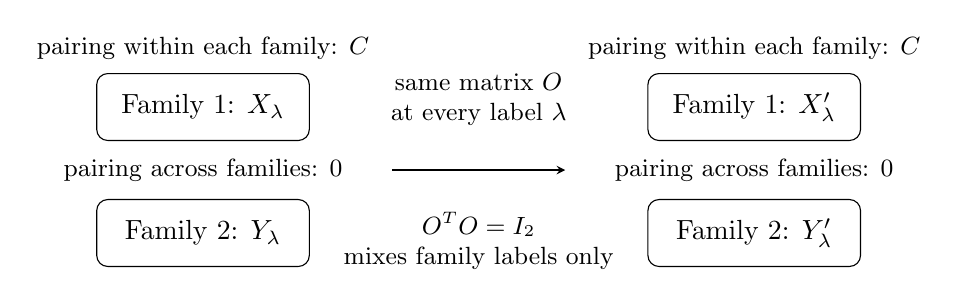
\begin{tikzpicture}[x=1cm,y=1cm,>=stealth,
 family/.style={draw,rounded corners,minimum width=2.7cm,minimum height=0.85cm}]
\node[family] (x) at (0,1.25) {Family 1: \(X_\lambda\)};
\node[family] (y) at (0,-0.35) {Family 2: \(Y_\lambda\)};
\node[font=\small,align=center] at (0,0.45) {pairing across families: \(0\)};
\node[font=\small] at (0,2.0) {pairing within each family: \(C\)};
\node[family] (xp) at (7,1.25) {Family 1: \(X'_\lambda\)};
\node[family] (yp) at (7,-0.35) {Family 2: \(Y'_\lambda\)};
\node[font=\small,align=center] at (7,0.45) {pairing across families: \(0\)};
\node[font=\small] at (7,2.0) {pairing within each family: \(C\)};
\draw[->] (2.4,0.45)--(4.6,0.45);
\node[align=center,font=\small] at (3.5,1.35)
 {same matrix \(O\)\\at every label \(\lambda\)};
\node[align=center,font=\small] at (3.5,-0.45)
 {\(O^TO=I_2\)\\mixes family labels only};
\end{tikzpicture}
\caption{Two formal copies of one pairing table. Each box represents a
whole family of symbols indexed by the same vertex--colour labels
\(\lambda\). The arrow denotes a change of formal variables, not a graph
edge or a physical operation. The joint table \(\widetilde C\), and hence
every Wick sum computed from it, is unchanged.}
\label{fig:copies}
\end{figure}

There is also an expression that detects the determinant of this change of
copy coordinates. For a vertex \(v\), choose distinct colours
\(\alpha_v,\beta_v\) and use \(X_{v,h}=X_{(v,h)}\),
\(Y_{v,h}=Y_{(v,h)}\). Form
\[
 \Delta_v=X_{v,\alpha_v}Y_{v,\beta_v}
             -X_{v,\beta_v}Y_{v,\alpha_v}.
\]
This is the determinant of the matrix with rows
\((X_{v,\alpha_v},X_{v,\beta_v})\) and
\((Y_{v,\alpha_v},Y_{v,\beta_v})\). Under a copy transformation \(O\)
it becomes \((\det O)\Delta_v\). A reflection, meaning an orthogonal
matrix of determinant \(-1\), changes the sign of a product of
\(\Delta_v\)'s on an odd set of vertices. If the remaining factors in
a moment are fixed by that reflection, invariance of the moment forces it
to vanish. Section~\ref{sec:higher} chooses those factors and the reflection
to obtain identities for the original source rows.

On an even set of vertices the product instead stays unchanged. This gives
the invariant pairing used in Section~\ref{sec:endpoint}. Its polynomial
dependence on auxiliary parameters is essential: degree comparisons turn
the symmetry constraints into exact identities. All parameter variations
take place in these auxiliary expressions, with the original edge weights
held fixed. We never assume that deleting vertices preserves the GHZ
condition.

\subsection{Shifted pairing sums and an alternating pairing}\label{sec:shifts}

For a row \(L\) on \(S\), replacing \(Z_{v,h}\) by
\(Z_{v,h}+L_v(h)\) adds a scalar to each formal symbol. We call \(L\)
the \emph{shift row}; the traditional word \emph{mean} will refer only to
these auxiliary scalars. For a fixed quadratic \(R\), define
\[
 \mathcal F_{S,R}(L)=
 \sum_{j=0}^{\lfloor |S|/2\rfloor}
       \frac{L^{|S|-2j}}{(|S|-2j)!}R^{[j]}\ \in\mathcal T_S.
\]
For any colour word \(\kappa\), expansion by the factors that supply a
scalar shift gives
\[
 [\kappa]\mathcal F_{S,R}(L)
 =\mathcal W_C\!\left(\prod_{v\in S}
       (Z_{v,\kappa(v)}+L_v(\kappa(v)))\right).
\]
Choose the shifted vertices, then pair the remaining vertices. This counts
each contribution once on both sides; the factorials on the left remove
the ordering of the selected row factors and edges. The odd and even cases
of this polynomial will be denoted by \(\Psi\) and \(E\), respectively,
in the following sections.

Fix an ordered pair of colours \((a,b)\). Define a local bilinear pairing
by
\[
 \epsilon(a,b)=1,\quad \epsilon(b,a)=-1,\quad
 \epsilon(a,a)=\epsilon(b,b)=0.
\]
On binary words, define
\[
 K_S(x^\kappa,x^\lambda)
   =\prod_{v\in S}\epsilon(\kappa(v),\lambda(v)),
\]
and extend bilinearly to coefficient arrays in \(\mathcal T_S\), first
projecting onto colours \(a,b\). Thus only complementary words contribute.
If \(\bar\kappa\) exchanges \(a\) and \(b\) in \(\kappa\), the
explicit formula is
\[
 K_S(F,G)=\sum_{\kappa:S\to\{a,b\}}
    (-1)^{|\kappa^{-1}(b)|}[\kappa]F[\bar\kappa]G.
\]
In particular, \(K_S(a^S,b^S)=1\) and
\(K_S(G,F)=(-1)^{|S|}K_S(F,G)\). The pairing is symmetric for even
\(|S|\) and alternating for odd \(|S|\). It is bilinear, not Hermitian.
We write \(K\) when the vertex set and ordered colour pair have been specified.

Expanding \(\prod_{v\in S}\Delta_v\) produces exactly these signs.
Together with the shifted-Wick identity, this explains why a simultaneous
copy transformation acts on both shift rows in
\(K_S(\mathcal F_{S,R}(L),\mathcal F_{S,R}(M))\). For even \(|S|\)
this polynomial is invariant under \(\mathrm O(2)\); for odd
\(|S|\) it is invariant under \(\mathrm{SO}(2)\).

All derivatives below are derivatives of finite polynomials in shift
parameters. For a polynomial map \(E\) on rows and fixed directions
\(J,J'\), our convention is
\[
 E_J(L)=\left.\frac{d}{dt}E(L+tJ)\right|_{t=0},\qquad
 E_{JJ'}(L)=\left.\frac{\partial^2}{\partial s\,\partial t}
       E(L+sJ+tJ')\right|_{s=t=0}.
\]
The underlying quadratic and all graph weights are held fixed.

\section{Vanishing identities after deleting one vertex}\label{sec:higher}

\subsection{Incident rows and their responses}\label{sec:rootrows}

A \emph{root} is a vertex singled out for a matching expansion. Delete a
root \(p\) from the original graph and put \(\Omega=V\setminus\{p\}\),
so \(|\Omega|=2m+1\). Decompose the edge polynomial as
\[
 A=R+\sum_{h\in\{a,b,c\}}x_{p,h}L_h^{(p)},\qquad
 L_h^{(p)}=\sum_{v\ne p}\sum_k A_{pv}(h,k)x_{v,k}.
\]
The quadratic \(R\) contains the edges avoiding \(p\); the row
\(L_h^{(p)}\) lists the ways to leave \(p\) with colour \(h\) at that
endpoint. The coefficient of \(x_{p,h}\) in the target equation is
\[
 L_h^{(p)}R^{[m]}=\tau_hh^\Omega.
\]
We call \(LR^{[m]}\) the \emph{response} of the row \(L\): it selects
one incident connection and matches the remaining vertices with edges of
\(R\). This use of ``response'' refers to a polynomial construction, not
to a physical susceptibility.

For odd \(p\), the higher response \(L^pR^{[(2m+1-p)/2]}\) inserts
\(p\) row factors and matches the other vertices through \(R\).
Here and in the next lemma \(p\) is an insertion count, not the name of
a graph vertex. These higher expressions are auxiliary identities; they
do not represent repeated physical use of a deleted root. The largest
insertion count, \(p=2m+1\), is called \emph{terminal}: its power of
\(R\) is zero.

The following lemma says that every higher response vanishes on every
binary word. Its proof has three ingredients: a reflection relates its
coefficients; rotations constrain the remaining common factor; finite
degree makes that factor constant.

\subsection{The vanishing lemma}
\begin{lemma}[Binary higher-response vanishing]\label{lem:higher}
Let \(\Omega\) have \(2m+1\ge3\) vertices, let \(R\) be an arbitrary quadratic
in \(\mathcal A_\Omega\), and let \(D\subseteq(\mathcal A_\Omega)_1\)
be a complex vector space of rows \(L\) such that
\begin{equation}
 \Phi(L)=L R^{[m]}=\sum_h f_h(L)h^\Omega.
 \tag{2}\label{eq:root}
\end{equation}
Here \(f_h:D\to\mathbb C\) extracts the pure colour coefficient of
\(\Phi(L)\). Assume all three \(f_h\) are nonzero functions and at least
two are linearly independent. For odd \(p\le2m+1\), define
\[
 H_p(L)=L^p R^{[(2m+1-p)/2]}.
\]
For every odd \(3\le p\le2m+1\), the tensor \(H_p(L)\) has zero coefficient on every word
using at most two colours, including the terminal degree \(p=2m+1\).
The same vanishing holds after polarization for products of arbitrary rows
from the same \(D\).
\end{lemma}

We will use ordinary polynomials in the coordinates of \(L\in D\).
If \(L=\sum_j t_jL_j\) in a basis of \(D\), this ring is
\(\mathbb C[D]=\mathbb C[t_1,\ldots,t_{\dim D}]\).
A nonzero coefficient function can be cancelled in this ring even if it
vanishes at some individual rows. Such cancellation is never performed
in the site algebra, which has zero divisors.

\begin{proof}
\emph{Pairing representation and reflection.}
Give formal variables \(X_{i,h}\) their \(R\) covariances, zero covariances
within a vertex, and give an auxiliary symbol \(\zeta\) covariance \(L_i(h)\) with
\(X_{i,h}\) and zero covariance with itself. A Wick moment with \(p\) copies
of \(\zeta\) and one specified coordinate at each vertex is the corresponding
coefficient of \(H_p(L)\). The \(p!\) assignments of auxiliary occurrences
are precisely those of the raw power \(L^p\); the divided power of \(R\)
counts each remaining matching once.

Duplicate this entire symbol family, including \(\zeta\), to obtain
\((X,\zeta_1)\), \((Y,\zeta_2)\) with zero cross-family pairings as in
Section~\ref{sec:twocopies}. The same copy matrix acts on every symbol,
including the two auxiliary symbols. Choose
distinct local colours \(\alpha_i,\beta_i\) at each vertex and set
\[
 \Delta_i=X_{i,\alpha_i}Y_{i,\beta_i}
              -X_{i,\beta_i}Y_{i,\alpha_i}.
\]
Over \(\mathbb C(s,t)\), the orthogonal reflection
\[
 \frac{1}{s^2+t^2}
 \begin{pmatrix}s^2-t^2&2st\\2st&t^2-s^2\end{pmatrix}
\]
fixes \(s\zeta_1+t\zeta_2\) and negates each \(\Delta_i\). It preserves the joint
covariance, so the moment of
\[
 (s\zeta_1+t\zeta_2)^{p+1}\prod_{i\in\Omega}\Delta_i
\]
is zero: there are an odd number of determinants. Extracting \(s^pt\)
and dividing by its nonzero binomial factor \(p+1\) gives
\begin{equation}
 \sum_{I\subseteq\Omega}(-1)^{|I|}H_p(L)(w_I)\Phi(L)(w'_I)=0,
 \tag{3}\label{eq:reflection}
\end{equation}
where \(w_I\) uses \(\beta\) on \(I\) and \(\alpha\) elsewhere, and \(w'_I\)
is complementary. The field \(\mathbb C(s,t)\) consists of rational
functions in two auxiliary parameters. The resulting identity is polynomial,
so it also holds when \(s^2+t^2=0\), where the displayed reflection has a
zero denominator. No operation on the original graph is being made.

\emph{A common pure factor and vanishing mixed coefficients.}
With constant local pair \(a,b\), \eqref{eq:reflection} says
\[
 f_b[a^\Omega]H_p=f_a[b^\Omega]H_p.
\]
Two independent \(f\)'s are coprime in \(\mathbb C[D]\), hence for
\(p=2r+1\) there is a common homogeneous polynomial \(q_r\) of degree
\(2r\) such that \([h^\Omega]H_p=f_hq_r\) for every \(h\); \(q_0=1\).
For a mixed word \(w\) avoiding an active colour \(h\), choose
\(\alpha_i=w_i\), \(\beta_i=h\). The only constant complementary word in
\eqref{eq:reflection} is \(h^\Omega\), giving \(f_h[w]H_p=0\). Polynomial
cancellation proves all binary mixed coefficients zero, even at individual
rows where \(f_h(L)=0\).

\emph{Rotation and finite degree.}
Define finite polynomials
\[
 \Psi(L)=\sum_{r=0}^m\frac{H_{2r+1}(L)}{(2r+1)!},
 \qquad
 g(L)=\sum_{r=0}^m\frac{q_r(L)}{(2r+1)!}.
\]
On any binary palette \(a,b\), the projection is therefore
\[
 \pi_{ab}\Psi(L)=g(L)\bigl(f_a(L)a^\Omega+f_b(L)b^\Omega\bigr).
\]
Use \(K=K_\Omega\) for the ordered colour pair \((a,b)\), as defined in
Section~\ref{sec:shifts}. The shifted symbols are
\(X_{i,h}+L_i(h)\) and \(Y_{i,h}+M_i(h)\). The shifted-Wick identity
shows that \(K(\Psi(L),\Psi(M))\) is invariant under simultaneous
\(\mathrm{SO}(2)\) rotation of the two shift rows: the joint pairing table
and each determinant are unchanged. Choose linearly independent
\(f_a,f_b\). This pairing is
\[
 \bigl(f_a(L)f_b(M)-f_b(L)f_a(M)\bigr)g(L)g(M).
\]
The determinant factor is a nonzero polynomial and is rotation invariant.
Cancel it in \(\mathbb C[D\times D]\), then rotate by \(45\) degrees and set
\(M=0\). Since \(g\) is even and \(g(0)=1\),
\[
 g(L/\sqrt2)^2=g(L).
\]
If \(g\) had positive degree, the degrees of the two sides would differ.
Thus \(g=1\), and all \(q_r\) with \(r\ge1\) vanish. Together with
\eqref{eq:reflection}, this proves whole binary vanishing through the
terminal degree \(2m+1\).

For completeness, \emph{polarization} here means substituting
\(L=t_1L_1+\cdots+t_pL_p\) and extracting the coefficient of
\(t_1\cdots t_p\). That coefficient in \(L^p\) is
\(p!L_1\cdots L_p\). Dividing by \(p!\ne0\) proves the stated vanishing
for products of arbitrary rows from the same \(D\); see also
\cite[Sections~4.4--4.5]{kraft} for this standard operation.
\end{proof}

For a matching polynomial satisfying \eqref{eq:target}, the incident rows
in Section~\ref{sec:rootrows} have responses
\(\tau_hh^{V\setminus\{p\}}\). Their span therefore satisfies
\eqref{eq:root} with three linearly independent \(f_h\). Thus
Lemma~\ref{lem:higher} applies at every original root, before diagonalization.

\section{Deleting a second vertex and eliminating bichromatic edges}\label{sec:diagonal}

We next extract the colour of one more vertex from the odd response.
The retained vertex set then has even size. The resulting identity says that
two incident-row insertions have zero pure coefficient. Applied to deletion
matching sums, this will force every aggregate bichromatic edge weight to zero.

\subsection{The identity after omitting a vertex}

\begin{lemma}[Even omission]\label{lem:omission}
In the setting of \eqref{eq:root}, omit a vertex \(q\), put
\(S=\Omega\setminus\{q\}\), and write
\[
 \begin{aligned}
 R&=Q+\sum_h h_q V_h,& L&=U+\sum_h d_hh_q,\\
 E(U)&=\sum_{r=0}^m\frac{U^{2r}}{(2r)!}Q^{[m-r]},&F&=E(0).
 \end{aligned}
\]
Here \(Q\) consists of edges of \(R\) lying in \(S\), and \(V_h\)
is the incident row at \(q\) in colour \(h\). The row \(U=U(L)\)
is \(L\) restricted to \(S\), while \(d_h=d_h(L)=L_q(h)\) is a scalar.
Thus \(E\) is the shifted matching polynomial \(\mathcal F_{S,Q}\)
from Section~\ref{sec:shifts}, and \(F=Q^{[m]}\) is its value with no
row insertions.
For any \(L_1,L_2\in D\) and any active colour \(k\),
\[
 [k^S]\,U(L_1)U(L_2)Q^{[m-1]}=0.
\]
This includes \(m=1\).
\end{lemma}

\begin{proof}
The full coefficient of \(q=h\) in \(\Psi(L)\) is
\[
 d_h E(U)+E_{V_h}(U),
\]
where the derivative convention is that of Section~\ref{sec:shifts},
with \(Q\) fixed. Fix the target colour \(k\) and choose another active
colour \(h\ne k\). Lemma~\ref{lem:higher} gives
\[
 \pi_{hk}\bigl(d_hE(U)+E_{V_h}(U)\bigr)=f_h(L)h^S.
\]
We use \(K=K_S\) with ordered colours \((h,k)\). By definition, its
arguments are projected by \(\pi_{hk}\); no identity of the omitted
three-colour coefficients is asserted.

Because \(|S|\) is even, \(K\) is symmetric and \(K(Z,h^S)=[k^S]Z\).
The same two-replica rotation gives
\begin{equation}
 \begin{aligned}
 K(E(U),E(U))&=K(F,E(\sqrt2U)),\\
 K(E(U),E_V(U))&=\frac{1}{\sqrt2}K(F,E_V(\sqrt2U)).
 \end{aligned}
 \tag{4}\label{eq:covariance}
\end{equation}
The second identity follows by differentiating the rotation identity at
shift rows \(U,U+tV\): the second rotated shift is zero at \(t=0\) and
\(E'(0)=0\). Substitute
\[
 \pi_{hk}E_{V_h}(U)=f_hh^S-d_h\pi_{hk}E(U)
\]
and the corresponding identity for \(\sqrt2L\) into the second equation
of \eqref{eq:covariance}. The first cancels the \(d_h\) terms, leaving
\[
 f_h(L)[k^S]\bigl(E(U)-F\bigr)=0.
\]
Cancel the nonzero polynomial \(f_h\). Separating homogeneous degrees and
polarizing yields
\begin{equation}
 [k^S]\,U(L_1)U(L_2)Q^{[m-1]}=0.
 \tag{5}\label{eq:omission}
\end{equation}
\end{proof}

\subsection{From deletion amplitudes to diagonal edge blocks}

For a fixed colour \(h\), a \emph{hafnian cofactor} is the matching
amplitude obtained by deleting two vertices in that colour. This name does
not assert an adjugate or inverse identity. We will prove the needed matrix
identity using the omission lemma. All matrices in the following proof have
their rows and columns indexed by the original vertex set \(V\).

\begin{lemma}[Global diagonal reduction]\label{lem:diagonal}
For every pair of vertices \(p,r\), the colour-indexed matrix
\((A_{pr}(i,h))_{i,h\in\{a,b,c\}}\) of a matching polynomial satisfying
\eqref{eq:target} is diagonal: \(A_{pr}(i,h)=0\) whenever \(i\ne h\).
\end{lemma}

\begin{proof}
For a fixed colour \(h\), define
\[
 \begin{aligned}
 M_h[p,r]&=A_{pr}(h,h) &&(p\ne r),& M_h[p,p]&=0,\\
 C_h[r,q]&=\operatorname{haf}\bigl(M_h[V\setminus\{r,q\}]\bigr)
                  &&(r\ne q),& C_h[q,q]&=0,\\
 B_{ih}[p,r]&=A_{pr}(i,h) &&(p\ne r),& B_{ih}[p,p]&=0.
 \end{aligned}
\]
Consider the colouring assigning \(i\) to \(p\) and \(h\) to every
other vertex. Expanding its matching sum at \(p\) gives
\[
 (B_{ih}C_h)[p,p]=\delta_{i,h}\tau_h.
\]
Here \(\delta_{i,h}\) is one if \(i=h\) and zero otherwise. To compute
the off-diagonal entries, take \(p\ne q\) and expand each
\(C_h[r,q]\) at its retained vertex \(p\):
\begin{equation}
 \begin{aligned}
 (B_{ih}C_h)[p,q]
 &=\sum_{\substack{r,s\in V\setminus\{p,q\}\\r\ne s}}
       A_{pr}(i,h)A_{ps}(h,h)\,
       \operatorname{haf}\bigl(M_h[V\setminus\{p,q,r,s\}]\bigr)\\
 &=0.
 \end{aligned}
 \tag{6}\label{eq:cofactor}
\end{equation}
The last expression is exactly \eqref{eq:omission} for two rows of the
original \(p\) family after omitting \(q\). Both sums are ordered; there
is no factor \(1/2\). Consequently
\[
 B_{ih}C_h=\delta_{i,h}\tau_h I.
\]
Taking \(i=h\) proves \(C_h\) invertible. Taking \(i\ne h\) then proves
\(B_{ih}=0\). Every original edge block is therefore diagonal. This uses
neither cofactor nonvanishing assumptions nor a change of basis.
\end{proof}

\section{The supported-edge identity}\label{sec:endpoint}

The preceding section proves Step 1 of Section~\ref{sec:overview}: only
monochromatic edges remain. We now prove Step 2. Fix a supported edge
\(pq\) in one colour. We must show that the matching subtotal containing
\(pq\) equals the entire amplitude of that colour.

The proof follows the two ways to match the roots: directly to one another,
or separately to retained vertices. The original equations constrain a
matrix recording these possibilities in two formal copies. Orthogonal
symmetry and the row identities restrict that matrix to an identity part
and a rank-one part. Two polynomial differential equations then determine
both parts, giving the required subtotal.

\subsection{Fixed graph data and the two-root expansion}

Let \(B,H\) be the symmetric zero-diagonal weight matrices for two active
colours after diagonal reduction. Write \(b_i,h_i\) for the corresponding
site variables at vertex \(i\); these are the two retained colours. Fix
roots \(p\ne q\), put \(S=V\setminus\{p,q\}\) and \(N=|S|\), and define
\[
 Q=\sum_{\substack{i<j\\i,j\in S}}(B_{ij}b_ib_j+H_{ij}h_ih_j).
\]
This is the original edge polynomial restricted to the retained vertices
and the two colours. It need not satisfy a GHZ condition. The fixed scalar
data are
\[
 \begin{aligned}
 d&=B_{pq},&e&=H_{pq},&\beta&=\mathrm{haf}(B),\\
 \eta&=\mathrm{haf}(H),&\alpha&=\mathrm{haf}(B[S]).
 \end{aligned}
\]
We assume \(d\ne0\), since \(pq\) is supported in colour \(B\).
The full amplitudes \(\beta,\eta\) are nonzero; \(e\) and the deletion
amplitude \(\alpha\) may vanish at this stage. The four fixed rows are
\[
\begin{array}{c|c|c|l}
\text{row}&\text{root}&\text{colour}&\text{definition on }S\\\hline
x&p&B&\displaystyle\sum_{i\in S}B_{pi}b_i\\
y&q&B&\displaystyle\sum_{i\in S}B_{qi}b_i\\
u&p&H&\displaystyle\sum_{i\in S}H_{pi}h_i\\
v&q&H&\displaystyle\sum_{i\in S}H_{qi}h_i
\end{array}
\]
For a shift row \(L\) on \(S\), set
\[
 E(L)=\mathcal F_{S,Q}(L)
 =\sum_{j=0}^{N/2}\frac{L^{2j}}{(2j)!}Q^{[N/2-j]},\qquad F=E(0).
\]
Each term pairs some retained vertices using \(Q\) and supplies a shift
factor at every remaining vertex. All row derivatives use the convention
of Section~\ref{sec:shifts}.

\begin{theorem}[Supported endpoint identity]\label{thm:endpoint}
Under the original target equation \eqref{eq:target} and the diagonal
reduction of Lemma~\ref{lem:diagonal}, every supported edge \(B_{pq}\ne0\)
in an active colour satisfies
\[
 \beta=B_{pq}\operatorname{haf}\bigl(B[V\setminus\{p,q\}]\bigr).
\]
\end{theorem}

\begin{lemma}[Two-root matching identities]\label{lem:boundary}
For arbitrary scalar parameters \(s,t,\lambda,\mu\), the fixed rows and
polynomial \(E\) above satisfy
\begin{equation}
 \begin{aligned}
 E_y(sx+tu)+dsE(sx+tu)&=s\beta b^S,\\
 E_v(sx+tu)+etE(sx+tu)&=t\eta h^S,\\
 E_x(\lambda y+\mu v)+d\lambda E(\lambda y+\mu v)&=\lambda\beta b^S,\\
 E_u(\lambda y+\mu v)+e\mu E(\lambda y+\mu v)&=\mu\eta h^S.
 \end{aligned}
 \tag{7}\label{eq:boundary}
\end{equation}
\end{lemma}

\begin{proof}
The original row at root
\(p\), restricted to the two colours, is
\(s(db_q+x)+t(eh_q+u)\). Apply Lemma~\ref{lem:higher} and extract the
colour \(b\) at the other root \(q\). A direct edge \(pq\) contributes
\(dsE(sx+tu)\). If \(q\) is matched into \(S\), its incident row
\(y\) is inserted, contributing \(E_y(sx+tu)\). The original pure
amplitude is \(s\beta\). This proves the first identity in \eqref{eq:boundary}.
Exchanging the colour or the two roots proves the other three identities.

The highest coefficient uses the terminal original odd response of degree
\(N+1\). All identities therefore hold in the full polynomial ring of shift
parameters, with the graph weights fixed.
\end{proof}

\begin{corollary}[Specialized row identities]\label{cor:specializations}
The same polynomial satisfies
\begin{equation}
 \begin{aligned}
 E_u(\lambda y)&=0,&E_v(sx)&=0,\\
 E_{yu}(sx)&=-dsE_u(sx),\\
 E_{uv}(sx)+eE(sx)&=\eta h^S,\\
 E_{xy}(0)+dF&=\beta b^S.
 \end{aligned}
 \tag{8}\label{eq:specializations}
\end{equation}
\end{corollary}

\begin{proof}
Set \(t=0\) in the second identity of \eqref{eq:boundary} and
\(\mu=0\) in the fourth to obtain the first line. Differentiate the
first two identities with respect to \(t\), then set \(t=0\), to obtain
the next two relations. Differentiating the first identity with respect
to \(s\) at \(s=t=0\) gives the last relation.
\end{proof}

\subsection{A matrix of two-copy insertion coefficients}

Use \(K=K_S\) with ordered colours \((b,h)\). It is symmetric because
\(N\) is even, and \(K(b^S,h^S)=1\). The polynomial
\(K(E(L_1),E(L_2))\) is invariant under the full \(\mathrm O(2)\) action
on the two shift rows. The Wick proof is as in Section~\ref{sec:higher}; a
determinant \(-1\) transformation contributes \((-1)^N=1\).

Group eight independent scalar indeterminates into four two-component
columns \(P,Q_c,R_c,S_c\). The subscript \(c\) labels a column; it is
not a graph colour. The entries specify coefficients in copies 1 and 2.
For \(i\in\{1,2\}\), define the shift row
\(L_i=P_i x+(Q_c)_iy+(R_c)_iu+(S_c)_iv\). The columns can later be
specialized to any complex values, including zero; they are not assumed
linearly independent. Define the scalar polynomials and matrices
\[
 \begin{aligned}
 G&=K(E(L_1),E(L_2)),& f&=G\big|_{R_c=S_c=0},\\
 M_{ij}&=\left.\partial_{(R_c)_i}\partial_{(S_c)_j}G\right|_{R_c=S_c=0},
 &T&=M+efI.
 \end{aligned}
\]
The entry \(M_{ij}\) records an insertion of the \(H\)-row \(u\) in
copy \(i\) and of the \(H\)-row \(v\) in copy \(j\). When both insertions
belong to the same copy, they represent the two roots being matched into
\(S\). There is one more possibility: the roots are matched directly to
each other by the \(H\)-edge of weight \(e\), leaving the retained
polynomial unchanged. That contribution is \(ef\) on each diagonal entry.
Thus the correction in \(T\) combines the two terms of the original
matching expansion, just as \(E_{uv}+eE\) does in
\eqref{eq:specializations}. There is no direct edge between distinct copies.

Here \(I=I_2\), and \(M,T\) are \(2\times2\) matrices whose indices
refer to copies, not graph vertices. We call \(T\) the corrected insertion
matrix. The scalar \(G\) is invariant when an orthogonal matrix \(O\)
acts on all four columns. Its differentiated matrix therefore satisfies
\[
 M(OP,OQ_c)=O M(P,Q_c)O^T,
\]
and similarly for \(T\). This transformation law is called matrix
\emph{covariance}; it differs from the pairing coefficients called
covariances earlier. By \eqref{eq:specializations},
\[
 M_{12}=K\bigl(E_u(P_1x+(Q_c)_1y),E_v(P_2x+(Q_c)_2y)\bigr)
\]
is divisible by \(P_1(Q_c)_2\); likewise \(M_{21}\) is divisible by
\(P_2(Q_c)_1\).

\subsection{The matrix form forced by symmetry and divisibility}

Use the bilinear dot product
\(P\cdot Q_c=P_1(Q_c)_1+P_2(Q_c)_2\), with no conjugation. The three
\emph{Gram coordinates} are the pairings of the two columns with themselves
and each other. The next lemma says that the insertion matrix has only two
scalar polynomial coefficients to determine. The matrix \(PQ_c^T\) is an
outer product and has rank at most one.

\begin{lemma}[Polynomial orthogonal kernel normal form]\label{lem:matrix}
For the corrected insertion matrix just defined,
\begin{equation}
 \begin{aligned}
 T&=\varphi I+\psi PQ_c^T,\\
 \varphi,\psi&\in\mathbb C[\sigma,\tau,\rho],\\
 \sigma&=P\cdot P,\qquad \tau=Q_c\cdot Q_c,\qquad \rho=P\cdot Q_c.
 \end{aligned}
 \tag{9}\label{eq:normalform}
\end{equation}
\end{lemma}

\begin{proof}[Proof sketch; complete proof in Appendix~\ref{app:normalform}]
The off-diagonal divisibility holds in every orthogonal coordinate system.
It implies that \(MP\) is parallel to \(P\) and \(M^TQ_c\) is parallel
to \(Q_c\). On the set where the needed bilinear products are nonzero,
these conditions give a scalar-identity part and one rank-one part.
The same divisibility makes their coefficients polynomials, so the identity
extends to all parameter values. Those scalar coefficients are invariant
under simultaneous orthogonal transformations. The classical scalar
invariant theorem then expresses them in the three Gram coordinates
\cite[Section~10.2(a)]{kraft}. Appendix~\ref{app:normalform} supplies both
the matrix argument and a direct proof of this scalar specialization.
\end{proof}

Orthogonal covariance alone would allow other matrices, for example
\(PP^T\). The divisibility obtained from the original matching equations
is what restricts the matrix to \eqref{eq:normalform}. The classical
invariant theorem is used only for its scalar coefficients.

\subsection{Finite polynomial degree determines the matrix}



\begin{lemma}[Polynomial differential equations]\label{lem:ode}
Let \(\mathcal R\) be a commutative integral domain, let \(d\in\mathcal R\) be nonzero,
and let \(p\in\mathcal R[z]\). If \(p'+dp=0\), then \(p=0\). If
\(p'+dp=k\) for \(k\in\mathcal R\), then \(p\) is constant and \(dp(0)=k\).
\end{lemma}

\begin{proof}
If \(p\ne0\) has degree \(r\), the coefficient of \(z^r\) in \(p'+dp\)
is \(d\) times the leading coefficient of \(p\), which is nonzero.
This excludes a homogeneous equation. In the inhomogeneous equation it
excludes \(r>0\); substituting a constant polynomial gives \(dp(0)=k\).
\end{proof}

The coefficient domain may itself be a polynomial ring. This elementary
step, including its endpoint cancellation consequence, is formalized in
\emph{PolynomialODE.lean}~\cite{lean}.

\begin{proof}[Proof of Theorem~\ref{thm:endpoint}]
We first eliminate the rank-one coefficient \(\psi\), then determine the
identity coefficient \(\varphi\). A subscript \(\rho\) denotes formal
partial differentiation in the Gram coordinate \(\rho\), with
\(\sigma,\tau\) held fixed.

\emph{The rank-one coefficient vanishes.}
At \((Q_c)_1=0\), differentiate \(M_{12}\) in \((Q_c)_1\) and use
\eqref{eq:specializations}. One obtains
\[
 \left.\partial_{(Q_c)_1}M_{12}\right|_{(Q_c)_1=0}
       =-dP_1\left.M_{12}\right|_{(Q_c)_1=0},
 \qquad P_1^2(Q_c)_2(\psi_\rho+d\psi)=0.
\]
The substitution
\[
 (\sigma,\tau,\rho)=\bigl(P_1^2+P_2^2,(Q_c)_2^2,P_2(Q_c)_2\bigr)
\]
is injective on polynomial rings: every \(\tau\ne0\) and arbitrary
\(\sigma,\rho\) is attained over \(\mathbb C\). Thus \(\psi_\rho+d\psi=0\).
Apply Lemma~\ref{lem:ode} over \(\mathbb C[\sigma,\tau]\), with polynomial
variable \(\rho\). Since \(d\ne0\), it gives \(\psi=0\), and hence \(T=\varphi I\).

\emph{The identity coefficient is constant.}
Write
\[
 Z=E_{uv}(P_2x+(Q_c)_2y)+eE(P_2x+(Q_c)_2y).
\]
The full expression is \(T_{22}=K(E(P_1x+(Q_c)_1y),Z)\). Differentiate
this expression in \((Q_c)_1\), then set \((Q_c)_1=0\).
Equation~\eqref{eq:boundary} gives
\[
 \left.\partial_{(Q_c)_1}T_{22}\right|_{(Q_c)_1=0}
 =P_1\beta K(b^S,Z)-dP_1\left.T_{22}\right|_{(Q_c)_1=0}.
\]
The pure-\(H\) coefficient of \(Z\) is \(\eta\): positive-degree \(B\)-colour row
insertions cannot contribute to an all-\(H\) word, so it is the same as
at zero, where \eqref{eq:specializations} gives
\(E_{uv}(0)+eF=\eta h^S\). Thus \(K(b^S,Z)=\eta\). Using
\eqref{eq:normalform} and the same injective substitution proves
\[
 \varphi_\rho+d\varphi=\beta\eta.
\]
Lemma~\ref{lem:ode}, again over \(\mathbb C[\sigma,\tau]\), gives
\(\varphi=\beta\eta/d\), independent of all three Gram variables. At the origin,
\[
 \varphi(0)=K(F,E_{uv}(0)+eF)=\eta K(F,h^S)=\eta\alpha.
\]
Since \(\eta\ne0\), this proves
\begin{equation}
 \beta=B_{pq}\operatorname{haf}\bigl(B[V\setminus\{p,q\}]\bigr)
 \qquad\text{whenever }B_{pq}\ne0.
 \tag{10}\label{eq:endpoint}
\end{equation}

Throughout the argument the edge weights are fixed. All differentiations are
in the auxiliary columns \(P,Q_c\), and the polynomial identities are finite.
\end{proof}

\section{Every colour is a perfect matching}\label{sec:matching}

\begin{corollary}[Matching rigidity of every active colour]\label{cor:matching}
Each active colour graph of a matching polynomial satisfying
\eqref{eq:target} is a weighted perfect matching.
\end{corollary}

\begin{proof}
The ordinary hafnian expansion at a vertex \(p\) says
\[
 \beta=\sum_{q\ne p}B_{pq}\operatorname{haf}\bigl(B[V\setminus\{p,q\}]\bigr).
\]
By \eqref{eq:endpoint}, every nonzero summand equals \(\beta\). Since
\(\beta\ne0\), the number of supported \(B\) neighbors of \(p\) is exactly
one. This holds at every vertex, and for each of the three colours by choosing
any other active colour as \(H\).
\end{proof}

\begin{corollary}[Disjoint colour matchings and unique contributions]\label{cor:unique}
The three colour matchings are pairwise edge-disjoint. Every vertex colouring
receives a contribution from at most one perfect matching.
\end{corollary}

\begin{proof}
Two such matchings cannot share an edge \(pq\): choosing that edge in colour
\(B\) and the other matching in colour \(H\) off \(p,q\) gives a mixed word
with nonzero coefficient, the product of nonzero matching weights.
Consequently their union is a simple cubic graph properly coloured with three
colours. Any prescribed vertex colouring supports at most one matching, because each
vertex has exactly one incident edge of its requested colour. Therefore a
mixed perfect matching would have a nonzero coefficient and violate
\eqref{eq:target}.
\end{proof}

\section{The remaining graph lemma}\label{sec:graph}

The following lemma is a special case of Bogdanov's obstruction
\cite{bogdanov}, also recorded in~\cite[Theorem~7]{cgi}. At this point, each colour is already a
perfect matching, and no vertex colouring can receive cancelling matching
contributions. We give an adapted version of Bogdanov's alternating-cycle
and minimal-arc proof for this special case.

\begin{lemma}[Three-matching obstruction]\label{lem:graph}
Three pairwise edge-disjoint perfect matchings \(F,G,H\) on \(n>4\) vertices
have a mixed perfect matching in their union.
\end{lemma}

\begin{proof}
Suppose otherwise. The union \(F\cup G\) must be a single alternating
Hamilton cycle \(C\), meaning a cycle visiting every vertex once:
otherwise choosing \(F\) on one component and \(G\)
on the others already gives a mixed matching. Label its vertices
\(0,\ldots,n-1\) cyclically. The matching \(H\) consists of chords, namely edges joining two
vertices of \(C\) that are not consecutive on it.

Figure~\ref{fig:chords} illustrates the next two constructions.
A chord with endpoints of opposite parity leaves two even paths when its
endpoints are deleted. Matching those paths along \(C\) and adding the chord
gives a mixed perfect matching. Hence all \(H\) chords join equal parities.
The two parity classes must each have even size; otherwise \(H\) is impossible.

An even-even chord and an odd-odd chord whose endpoints interlace (occur alternately around the cycle) leave four
even paths on deleting their endpoints. Those paths and the two chords give
a mixed perfect matching when \(n>4\). Thus no such pair interlaces.

Choose a chord and one of its sides with the fewest vertices strictly inside,
over all chords and both sides. Its endpoints have equal parity, so its
interior contains a vertex of the opposite parity. Every vertex of that
opposite parity in the interior must be \(H\)-matched to another interior
vertex; a partner outside would give an interlacing opposite-parity chord.
Therefore some \(H\) chord lies strictly inside the chosen arc. One side of
that chord has fewer interior vertices, a contradiction.
\end{proof}

\begin{figure}[htbp]
\centering
\begin{minipage}[t]{0.48\textwidth}
\centering
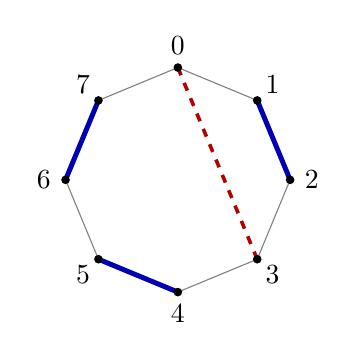
\begin{tikzpicture}[scale=0.92]
\foreach \v in {0,...,7} {
 \coordinate (v\v) at ({90-45*\v}:1.55);
 \node at ({90-45*\v}:1.85) {\(\v\)};
}
\draw[gray] (v0)--(v1)--(v2)--(v3)--(v4)--(v5)--(v6)--(v7)--cycle;
\draw[blue!70!black,line width=1.8pt] (v1)--(v2) (v4)--(v5) (v6)--(v7);
\draw[red!70!black,dashed,line width=1.3pt] (v0)--(v3);
\foreach \v in {0,...,7} \fill (v\v) circle (1.7pt);
\end{tikzpicture}

\small (a) One opposite-parity chord:\\
\(H:\{03\}\), cycle edges \(\{12,45,67\}\).
\end{minipage}\hfill
\begin{minipage}[t]{0.48\textwidth}
\centering
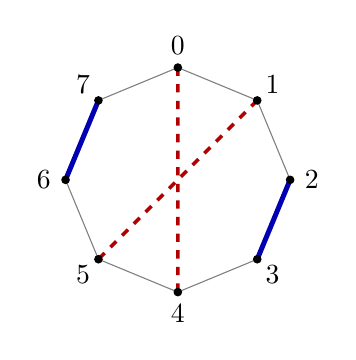
\begin{tikzpicture}[scale=0.92]
\foreach \v in {0,...,7} {
 \coordinate (v\v) at ({90-45*\v}:1.55);
 \node at ({90-45*\v}:1.85) {\(\v\)};
}
\draw[gray] (v0)--(v1)--(v2)--(v3)--(v4)--(v5)--(v6)--(v7)--cycle;
\draw[blue!70!black,line width=1.8pt] (v2)--(v3) (v6)--(v7);
\draw[red!70!black,dashed,line width=1.3pt] (v0)--(v4) (v1)--(v5);
\foreach \v in {0,...,7} \fill (v\v) circle (1.7pt);
\end{tikzpicture}

\small (b) Interlacing equal-parity chords:\\
\(H:\{04,15\}\), cycle edges \(\{23,67\}\).
\end{minipage}
\caption{Two ways to construct a mixed perfect matching, illustrated on
an eight-cycle. Dashed edges belong to \(H\); heavy solid edges are chosen
from the cycle \(F\cup G\). Together they cover every vertex exactly once.
Only the selected \(H\)-edges are drawn. The crossing in (b) is not a vertex.
These are local configurations used in the proof, not GHZ constructions.}
\label{fig:chords}
\end{figure}

This supplies a mixed perfect matching, contradicting Section~\ref{sec:matching}.
Equation~\eqref{eq:target} is impossible for every even \(n>4\), completing
the proof of Theorem~\ref{thm:main}. The graph interpretation in
Section~\ref{sec:model} and restriction to three active colours now give
Theorem~\ref{thm:graphmain}.

\section{Boundary cases and formal verification}\label{sec:scope}

For \(n=4\), the three matchings of \(K_4\) give the permitted ternary
source. In Section~\ref{sec:graph}, a pair of interlacing chords then exhausts
the vertices and gives the pure third matching, so no contradiction is asserted.
Sections~\ref{sec:higher}--\ref{sec:matching} remain valid at \(n=4\), including
their terminal response coefficients. For \(n=2\), the odd-core lemma does not
apply and arbitrary target dimension is possible. Odd \(n\) has no perfect
matchings in this model.

The normalized equation-system statement is formalized in Lean for every
even \(N\ge6\) and every \(D\ge3\), with arbitrary complex aggregate
endpoint-colour weights~\cite{lean}. The real-weight transfer is also checked.
Lemma~\ref{lem:normalization} and the aggregation in
Section~\ref{sec:overview} explain the mathematical bridge to the graph
statement used here. Appendix~\ref{app:formal} gives the exact theorem,
verification boundary, reproduction commands, and written-proof provenance.

\appendix
\section{Polynomial form of the insertion matrix}\label{app:normalform}

This appendix supplies the coordinate details deferred from
Lemma~\ref{lem:matrix}. Every pairing and orthogonal frame below uses the
complex bilinear dot product defined in Section~\ref{sec:endpoint}.

\begin{proof}[Proof of Lemma~\ref{lem:matrix}]
In an orthonormal frame where \(P_1=0\), \(M_{12}=0\), so \(MP\) is parallel
to \(P\). In a frame where \((Q_c)_2=0\), \(M_{12}=0\), so \(M^TQ_c\) is
parallel to \(Q_c\). Such frames exist when the relevant bilinear square is nonzero. We first
work on the set where these squares and the required determinants are nonzero. Their eigenvalues agree when \(P\cdot Q_c\ne0\). For two independent
columns in dimension two, these conditions force
\[
 M=\varphi_0I+\psi PQ_c^T.
\]
Indeed, \(M\) minus the common eigenvalue times \(I\) annihilates \(P\) and
has left kernel \(Q_c\); its rank-one form is a multiple of
\((P\cdot Q_c)I-PQ_c^T\). The off-diagonal divisibility proved in the main text shows that
\[
 \psi=\frac{M_{12}}{P_1(Q_c)_2},\qquad \varphi_0=M_{11}-\psi P_1(Q_c)_1
\]
are polynomials. The resulting identity, proved whenever the excluded
polynomials are nonzero, therefore holds identically, including at their zeros.
Uniqueness and covariance make \(\varphi_0,\psi\) scalar \(\mathrm O(2)\) invariants,
and the same is true of \(\varphi=\varphi_0+ef\).

The scalar invariant-ring assertion is the two-vector case of the first
fundamental theorem for the orthogonal group; see~\cite[Section~10.2(a)]{kraft}.
For completeness, we prove this particular case directly. In coordinates
\(p_+=P_1+\mathrm iP_2\), \(p_-=P_1-\mathrm iP_2\), and
\(q_\pm=(Q_c)_1\pm\mathrm i(Q_c)_2\), where \(\mathrm i^2=-1\),
a matrix in \(\mathrm{SO}(2)\) multiplies the plus coordinates by a
nonzero scalar \(z\) and the minus coordinates by \(z^{-1}\). Its invariant monomials
are generated by \(\sigma,\tau,r=p_+q_-,s=p_-q_+\), with
\(rs=\sigma\tau\). Reflection exchanges \(r,s\). Symmetric polynomials
reduce to \(r+s=2\rho\) and \(rs=\sigma\tau\), giving
\(\mathbb C[\sigma,\tau,\rho]\). There is no polynomial relation among the three Gram coordinates:
when \(\tau\ne0\), choose \(Q_c=(0,\sqrt\tau)^T\),
\(P_2=\rho/\sqrt\tau\), and \(P_1^2=\sigma-\rho^2/\tau\).
This realizes arbitrary \(\sigma,\rho\); a polynomial relation would
therefore vanish identically.
\end{proof}

\section{Formal artifact and proof provenance}\label{app:formal}

The historical sources collected in~\cite{review}
are internal research notes from this repository. Their proofs have been
included here, so these citations identify provenance rather than replace
mathematical steps. The published external inputs are the graph formulation
and combinatorial obstruction~\cite{kgs,cgi}; the pairing and invariant-theory
references~\cite{isserlis,kraft} provide background for identities also proved
in the text.

The Lean development in~\cite{lean} proves nonexistence for every even
\(N\ge6\) and every \(D\ge3\), with arbitrary complex aggregate
endpoint-colour weights and the normalized equations
\[
 W(\kappa)=
 \begin{cases}
  1,&\kappa\text{ is constant},\\
  0,&\kappa\text{ is mixed}.
 \end{cases}
\]
The final declaration is
\texttt{UpstreamFullProof.eqSystem\_no\_solution\_ge6\_ge3}
in \texttt{FullProof.lean}, within the namespace \texttt{KrennAllOrders}.
An adapter identifies the local matching sums with the exact
\texttt{MonochromaticQuantumGraph.WeightsN} and \texttt{EqSystemN}
definitions in the pinned Formal Conjectures source. The final theorem
has no remaining source-reduction or structural hypothesis.

The checked proof covers the complete chain: the matching model, copy
symmetries, response and omission identities, diagonal reduction, the
polynomial kernel argument, the supported-edge identity, and the graph
obstruction. The real-to-complex transfer and the corresponding real-weight
corollaries are also formalized.

The dependency audit reports only three standard axioms:
\texttt{propext}, \texttt{Classical.choice}, and \texttt{Quot.sound}.
There are no proof holes or additional axioms in the final dependencies.

The final Lean statement uses aggregate weights and unit pure amplitudes.
Sections~\ref{sec:overview} and~\ref{sec:normalization} give the explicit
mathematical translations from the multigraph formulation and arbitrary
nonzero pure amplitudes used here. These explanatory translations should
be distinguished from the exact interface of the linked Lean theorem.
The artifact includes the pinned toolchain, source hashes, axiom reports,
and commands for reproducing both the local proof and the upstream adapter.

For the local proof, install Lean through \texttt{elan} and run from the
repository root:
\begin{verbatim}
cd formal/all-orders
lake exe cache get
python3 verify.py
\end{verbatim}
The toolchain is Lean 4.33.1; the package manifest fixes its mathlib dependency.
To check the exact upstream interface, prepare the Formal Conjectures checkout
at the revision recorded in \texttt{formal/upstream-adapter/README.md}, then run
from the repository root:
\begin{verbatim}
cd formal/upstream-adapter
python3 verify.py --upstream /path/to/formal-conjectures
\end{verbatim}
This second command checks the pinned upstream revision and compiles the
adapter, final complex theorem, and real corollaries. The linked reproduction
instructions in~\cite{lean} specify the checkout and cache commands in full.

The written argument is based on the frozen mathematical source
in~\cite{review}. The associated agent audits are internal research records;
they do not constitute external peer review. This manuscript develops its
exposition independently of those historical records.

\begingroup
\small
\raggedright
\begin{thebibliography}{99}

\bibitem{kgz}
Mario Krenn, Xuemei Gu, and Anton Zeilinger.
Quantum experiments and graphs: Multiparty states as coherent superpositions
of perfect matchings. \emph{Physical Review Letters}, 119:240403, 2017.
\href{https://doi.org/10.1103/PhysRevLett.119.240403}{doi:10.1103/PhysRevLett.119.240403}.

\bibitem{graphs2}
Xuemei Gu, Manuel Erhard, Anton Zeilinger, and Mario Krenn.
Quantum experiments and graphs II: Quantum interference, computation,
and state generation. \emph{Proceedings of the National Academy of Sciences},
116:4147--4155, 2019.
\href{https://doi.org/10.1073/pnas.1815884116}{doi:10.1073/pnas.1815884116}.

\bibitem{bogdanov}
Ilya Bogdanov.
Answer to ``Graphs with only disjoint perfect matchings.''
MathOverflow, April 12, 2017.
\href{https://mathoverflow.net/a/267013}{Original answer}.

\bibitem{cgclass}
L. Sunil Chandran and Rishikesh Gajjala.
Edge-coloured graphs with only monochromatic perfect matchings and their
connection to quantum physics.
\emph{Electronic Journal of Combinatorics}, 33(3):P3.21, 2026.
\href{https://doi.org/10.37236/12573}{doi:10.37236/12573}.

\bibitem{sixvertex}
Algal (repository maintainer).
A Lean proof of the Krenn--Gu \((6,3)\) case. Public formal proof artifact, 2026.
\href{https://github.com/algal/krenn-gu-6x3-certificate}{Source and verification documentation}.
Accessed September 26, 2026; this manuscript does not independently rebuild
that external artifact.

\bibitem{krennstatus}
Mario Krenn.
Inherited vertex coloring of graphs. Author's problem and progress page,
May and July 2026 updates.
\href{https://mariokrenn.wordpress.com/graph-theory-question/}{Progress announcement}.
Accessed September 26, 2026.

\bibitem{nexus}
George Tsoukalas et al.
Advancing mathematics research with AI-driven formal proof search.
arXiv:2605.22763v2, June 8, 2026.
\href{https://arxiv.org/abs/2605.22763v2}{Primary preprint}.
Reference 38 lists the related tensor-algebraic no-go manuscript as in preparation.

\bibitem{kgs}
Mario Krenn, Xuemei Gu, and D\'aniel Solt\'esz.
Questions on the structure of perfect matchings inspired by quantum physics.
In \emph{Proceedings of the 2nd Croatian Combinatorial Days}, pages 57--70, 2019.
\href{https://doi.org/10.5592/CO/CCD.2018.05}{doi:10.5592/CO/CCD.2018.05}.
\href{https://arxiv.org/abs/1902.06023v2}{arXiv:1902.06023v2}.

\bibitem{cgi}
L. Sunil Chandran, Rishikesh Gajjala, and Abraham M. Illickan.
Krenn--Gu conjecture for sparse graphs.
In \emph{49th International Symposium on Mathematical Foundations of Computer
Science (MFCS 2024)}, volume 306 of LIPIcs, pages 41:1--41:15.
Schloss Dagstuhl--Leibniz-Zentrum f\"ur Informatik, 2024.
\href{https://doi.org/10.4230/LIPIcs.MFCS.2024.41}{doi:10.4230/LIPIcs.MFCS.2024.41}.
\href{https://arxiv.org/abs/2407.00303v1}{arXiv:2407.00303v1}.
Theorem 7 records the obstruction attributed to Ilya Bogdanov.

\bibitem{cg}
L. Sunil Chandran and Rishikesh Gajjala.
Graph-theoretic insights on the constructability of complex entangled states.
\emph{Quantum}, 8:1396, 2024.
\href{https://doi.org/10.22331/q-2024-07-03-1396}{doi:10.22331/q-2024-07-03-1396}.

\bibitem{logic}
Alba Cervera-Lierta, Mario Krenn, and Al\'an Aspuru-Guzik.
Design of quantum optical experiments with logic artificial intelligence.
\emph{Quantum}, 6:836, 2022.
\href{https://doi.org/10.22331/q-2022-10-13-836}{doi:10.22331/q-2022-10-13-836}.

\bibitem{isserlis}
L. Isserlis.
On a formula for the product-moment coefficient of any order of a normal
frequency distribution in any number of variables.
\emph{Biometrika}, 12(1--2):134--139, 1918.
\href{https://doi.org/10.1093/biomet/12.1-2.134}{doi:10.1093/biomet/12.1-2.134}.

\bibitem{kraft}
Hanspeter Kraft and Claudio Procesi.
\emph{Classical Invariant Theory: A Primer}.
Preliminary version, July 1996.
Section 10.2(a), page 114: the first fundamental theorem for the orthogonal group.
\href{https://dmi.unibas.ch/fileadmin/user_upload/dmi/Personen/Kraft_Hanspeter/Classical_Invariant_Theory.pdf}{Authors' manuscript}.

\bibitem{review}
Krenn--Gu research repository.
Complete all-orders proof and internal review record, September 26, 2026.
\href{https://github.com/rrajasek95/krenn-conjecture/blob/e66211d22978927f1c761997472fa9f5cf8f9421/proofs/krenn-gu-all-orders-two-replica-proof.md}{Frozen mathematical source} and
\href{https://github.com/rrajasek95/krenn-conjecture/blob/e66211d22978927f1c761997472fa9f5cf8f9421/notes/all-orders-two-replica-review-2026-09-26.md}{internal review and provenance record}.

\bibitem{lean}
Krenn--Gu research repository.
Complete Lean formalization of the normalized Krenn--Gu equation system.
Lean 4.33.1 source and verification records, September 26, 2026.
\href{https://github.com/rrajasek95/krenn-conjecture/blob/5e7d0fe0b6058f4658ccc5dae5f148ea8e7bc248/formal/upstream-adapter/FullProof.lean}{Exact complex theorem},
\href{https://github.com/rrajasek95/krenn-conjecture/blob/5e7d0fe0b6058f4658ccc5dae5f148ea8e7bc248/formal/upstream-adapter/RealCorollaries.lean}{real transfer and corollaries},
\href{https://github.com/rrajasek95/krenn-conjecture/blob/5e7d0fe0b6058f4658ccc5dae5f148ea8e7bc248/formal/all-orders/README.md}{proof chain and reproduction instructions}, and
\href{https://github.com/rrajasek95/krenn-conjecture/blob/5e7d0fe0b6058f4658ccc5dae5f148ea8e7bc248/formal/upstream-adapter/verification.json}{upstream verification metadata}.


\end{thebibliography}
\endgroup
\end{document}
